\documentclass[border=2pt]{standalone}
\usepackage{tikz,pgfplots}
\usetikzlibrary{quotes,angles}
\pgfplotsset{compat=1.17}
\begin{document}
\begin{tikzpicture}
  \draw
    (4,3) coordinate (B) node[right] {$B$}
    -- node[above right] {$r$} (1,2) coordinate (A) node[left] {$A$}
    -- node[above] {$r$} (3.0981,4.3660) coordinate (C) node[above right] {$B^{\prime}$}
    pic["$\theta$", draw=blue, <->, angle eccentricity=1.2, angle radius=1cm]
    {angle=B--A--C};
    
   \draw[->] (-.25,1)--(5,1) node[below]{$x$};
   \draw[->] (0,0.75)--(0,5) node[left]{$y$};
\end{tikzpicture}
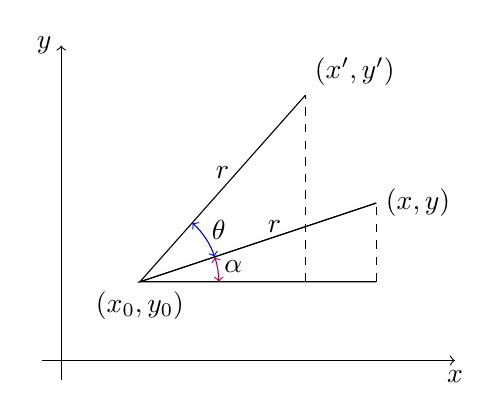
\begin{tikzpicture}
  \draw
    (4,3) coordinate (B) node[right] {$(x,y)$}
    -- node[above right] {$r$} (1,2) coordinate (A) node[anchor=north] {$(x_0,y_0)$}
    -- node[above] {$r$} (3.0981,4.3660) coordinate (C) node[anchor=south west] {$(x^{\prime},y^{\prime})$}
    pic["$\theta$", draw=blue, <->, angle eccentricity=1.2, angle radius=1cm]
    {angle=B--A--C};
    
    \draw
    (4,3) coordinate (BB)
    -- (1,2) coordinate (AA)
    -- (4,2) coordinate (CC)
    pic["$\alpha$", draw=purple, <->, angle eccentricity=1.2, angle radius=1cm]
    {angle=CC--AA--BB};
    
   \draw[dashed] (1,2)--(4,2);    
   \draw[dashed] (3.0981,2)--(3.0981,4.3660);
   \draw[dashed] (4,2)--(4,3);    
  \draw[->] (-.25,1)--(5,1) node[below]{$x$};
   \draw[->] (0,0.75)--(0,5) node[left]{$y$};
\end{tikzpicture}
\end{document}